\documentclass[12pt,letterpaper]{exam}
\usepackage[lmargin=1in,rmargin=1in,tmargin=1in,bmargin=1in]{geometry}
\usepackage{../style/exams}

% -------------------
% Course & Exam Information
% -------------------
\newcommand{\course}{MAT 108: Exam 3}
\newcommand{\term}{Fall -- 2021}
\newcommand{\examdate}{12/16/2021}
\newcommand{\timelimit}{85 Minutes}

\setbool{hideans}{false} % Student: True; Instructor: False

% -------------------
% Content
% -------------------
\begin{document}

\examtitle
\instructions{Write your name on the appropriate line on the exam cover sheet. This exam contains \numpages\ pages (including this cover page) and \numquestions\ questions. Check that you have every page of the exam. Answer the questions in the spaces provided on the question sheets. Be sure to answer every part of each question and show all your work. If you run out of room for an answer, continue on the back of the page --- being sure to indicate the problem number.} 
\scores
\bottomline
\newpage

% ---------
% Questions
% ---------
\begin{questions}

% Question 1
\newpage
\question The probabilities of several events in a finite probability space are given below:
	\[
	\begin{aligned}
	P(A)&= 0.60 & P(C)&= 0.35 \\
	P(B)&= 0.45 & P(D)&= 0.80 \\
	P(B \text{ and }D)&= 0.50 & P(D \;|\;C)&= 0.70
	\end{aligned}
	\]

\begin{parts}
\part[3] Assuming $A$ and $B$ are independent events, find $P(A \text{ or } B)$.
\part[1] Assume $A$ and $C$ are disjoint events. Find $P(A \text{ or }C)$.
\part[3] Can $A$ and $C$ be independent events? Explain.
\part[2] Find $P(C \text{ and } D)$. 
\part[3] Find $P(B \;|\; D)$. Can $B$ and $D$ be independent? Explain. 
\part[3] Can $A$ and $D$ be disjoint events? Explain. 
\end{parts} \pspace

{\noindent\bfseries Solution.}

\begin{enumerate}[(a)]
\item Because $A$ and $B$ are independent, then $P(A \text{ and } B)= P(A) \cdot P(B)= 0.60 \cdot 0.45= 0.27$. But then\dots
	\[
	P(A \text{ or } B)= P(A) + P(B) - P(A \text{ and } B)= 0.60 + 0.45 - 0.27= 0.78
	\] \vfill

\item Because $A$ and $C$ are disjoint, we know $P(A \text{ and }C)= 0$. But then
	\[
	P(A \text{ or } C)= P(A) + P(C) - P(A \text{ and } C)= 0.60 + 0.35 - 0= 0.95
	\] \vfill

\item No. Because we are assuming $A$ and $C$ are disjoint events, $A$ and $C$ cannot be independent because disjoint events are never independent. \vfill

\item 
	\[
	P(C \text{ and } D)= P(C) \cdot P(D \;|\; C)= 0.35 \cdot 0.70= 0.245
	\] \vfill

\item We know that $B$ and $D$ cannot be independent because if they were, then we would have $P(B \text{ and } D)= P(B) \cdot P(D)$. However, $P(B) \cdot P(D)= 0.45 \cdot 0.80= 0.36 \neq 0.50= P(B \text{ and } D)$. Now we have\dots
	\[
	P(B \;|\; D)= \dfrac{P(B \text{ and }D)}{P(D)}= \dfrac{0.50}{0.80}= 0.625
	\] \vfill

\item No. If $A$ and $B$ were disjoint, then $P(A \text{ or } B)= P(A) + P(B)$. But $P(A) + P(B)= 0.60 + 0.45= 1.05 > 1$, which is impossible. \vfill
\end{enumerate}





% Question 2
\newpage
\question In a post-apocalyptic world, Santa is making a list and checking it twice. Of course, the list consists of all the types of people in the world: naughty, nice, and Jeff Goldblum. A breakdown of the people across the populated continents is given below:
	\begin{table}[!ht]
	\centering
	\begin{tabular}{|r||c|c|c|c|c||c|} \hline
	& North America & South America & Europe & Asia & Africa & Total \\ \hline
	Naughty & $955$ & $857$ & $778$ & $3250$ & $1350$ & $7190$ \\ \hline
	Nice & $623$ & $706$ & $795$ & $5201$ & $1066$ & $8391$ \\ \hline
	Jeff Goldblum & $1$ & $0$ & $0$ & $0$ & $0$ & $1$ \\ \hline \hline
	Total & $1579$ & $1563$ & $1573$ & $8451$ & $2416$ & $15582$ \\ \hline
	\end{tabular}
	\end{table}

\begin{parts}
\part[2] Find the probability that a randomly selected person is from Asia. 
\part[2] Find the probability that a randomly selected person was naughty.
\part[2] Find the probability that a randomly selected person was a nice person from Europe.
\part[2] Find the probability that a randomly selected person from North America was Jeff Goldblum. 
\part[2] Find the probability that a randomly selected person from South America or Africa was nice. 
\end{parts} \pspace

{\noindent\bfseries Solution.}

\begin{enumerate}[(a)]
\item 
	\[
	P(\text{Asia})= \dfrac{8451}{15582} \approx 0.5424
	\] \vfill

\item 
	\[
	P(\text{Naughty})= \dfrac{7190}{15582} \approx 0.4614
	\] \vfill

\item 
	\[
	P(\text{Nice and Europe})= \dfrac{795}{15582} \approx 0.0510
	\] \vfill

\item 
	\[
	P(\text{Jeff Goldblum | North America})= \dfrac{1}{1579} \approx 0.0006
	\] \vfill

\item 
	\[
	P(\text{Nice | South America or Africa})= \dfrac{706 + 1066}{1563 + 2416}= \dfrac{1772}{3979} \approx 0.4453
	\] \vfill
\end{enumerate}





% Question 3
\newpage
\question A class was polled on whether they liked dogs, cats, or neither. Of the 16 students in the room, eight (correctly) preferred dogs, three (incorrectly) preferred cats, and one student (partially correctly) could not decide between the two and said that they preferred both. Find the probability that a randomly selected student\dots
        \begin{parts}
        \part[3] \dots preferred either dogs or cats.
        \part[3] \dots preferred neither dogs nor cats.
        \part[3] \dots preferred only dogs.
        \part[3] \dots did not prefer cats.
        \part[3] \dots that preferred dogs also enjoyed cats. 
        \end{parts} \pspace
	\[
	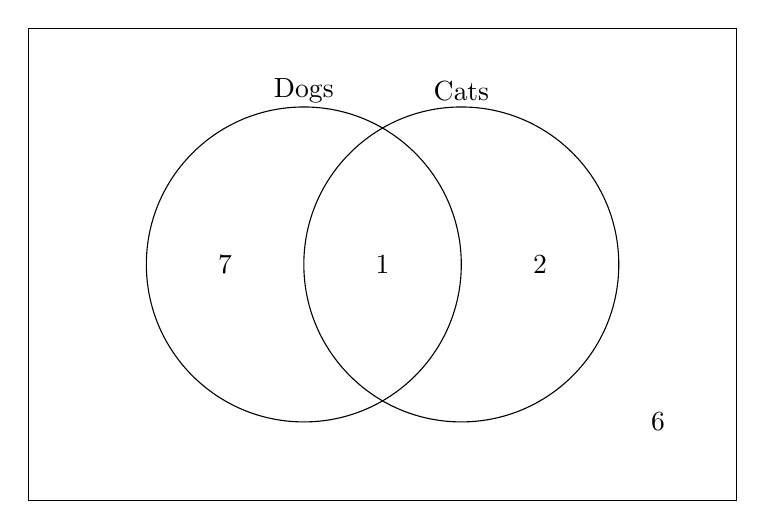
\begin{tikzpicture}
	\draw (0,0) rectangle (9,6);
	\draw (3.5,3) circle (2);
	\draw (5.5,3) circle (2);
	
	\node at (3.5,5.2) {Dogs};
	\node at (5.5,5.2) {Cats}; 
	
	\node at (2.5,3) {7};
	\node at (4.5,3) {1};
	\node at (6.5,3) {2};
	\node at (8,1) {6};
	\end{tikzpicture}
	\]

{\noindent\bfseries Solution.}

\begin{enumerate}[(a)]
\item 
	\[
	\begin{aligned}
	P(\text{Dogs or Cats})&= \dfrac{7 + 1 + 2}{16}= \dfrac{10}{16} \approx 0.6250 \\
	\text{OR} \\
	P(\text{Dogs or Cats})&= \dfrac{8 + 3 - 1}{16}= \dfrac{10}{16} \approx 0.6250
	\end{aligned}
	\] \vfill

\item 
	\[
	P(\text{Neither Cats nor Dogs})= \dfrac{6}{16} \approx 0.375
	\] \vfill

\item 
	\[
	P(\text{Only Dogs})= \dfrac{7}{16} \approx 0.4375
	\] \vfill

\item 
	\[
	P(\text{Not Cats})= \dfrac{7 + 6}{16}= \dfrac{13}{16} \approx 0.8125
	\] \vfill

\item 
	\[
	P(\text{Cats | Dogs})= \dfrac{1}{7 + 1}= \dfrac{1}{8} \approx 0.125
	\] \vfill
\end{enumerate}





% Question 4
\newpage
\question It is the holiday season and a popular topic of conversation are the actors and actresses of Hollywood. Of mothers across the country, only 40\% know the actor Benedict Cumberbatch. Mothers that know the actor pronounce his name correctly only 50\% of the time---the rest referring to him as `Bernadette Kamberbench.' For mothers that do not know the actor, only 30\% pronounce his name correctly---the rest calling him `Barnacle Clampersnatch.' Find the probability that a randomly selected mother\dots

\begin{parts}
\part[3] \dots will know Benedict Cumberbatch.
\part[3] \dots will know Benedict Cumberbatch and correctly pronounce his name.
\part[3] \dots will correctly pronounce Benedict Cumberbatch's name.
\part[3] \dots will know Benedict Cumberbatch or pronounce his name correctly.
\part[3] \dots that mispronounces Benedict Cumberbatch's name will refer to him as `Barnacle Clampersnatch.'
\end{parts}
	\[
	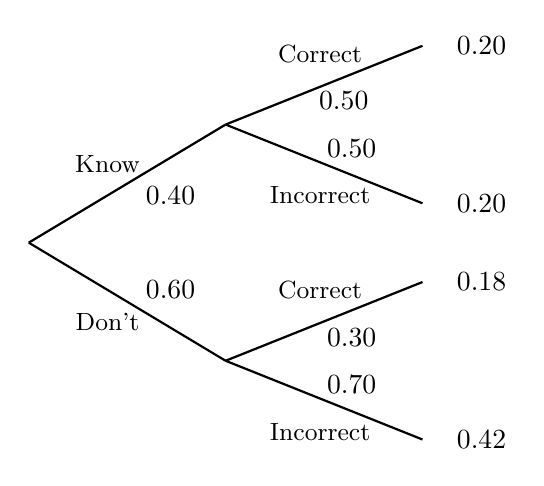
\begin{tikzpicture}[scale= 1.0]
	\def\FirstUpLabel{\small Know}
	\def\FirstDownLabel{\small Don't}
	\def\SecondUpLabel{\small Correct}
	\def\SecondDownLabel{\small Incorrect}
	\def\Up{$0.40$}
	\def\Down{$0.60$}
	\def\UpUp{$0.50$}
	\def\UpDown{$0.50$}
	\def\DownUp{$0.30$}
	\def\DownDown{$0.70$}
	\def\first{$0.20$}
	\def\second{$0.20$}
	\def\third{$0.18$}
	\def\fourth{$0.42$}
	
	\node at (1,1) {\FirstUpLabel};	
	\node at (1,-1) {\FirstDownLabel};	
	\node at (1.8,0.6) {\Up};
	\node at (1.8,-0.6) {\Down};
	\draw[thick] (0,0) -- (2.5,1.5);
	\draw[thick] (0,0) -- (2.5,-1.5);
	
	\node at (3.7,2.4) {\SecondUpLabel};
	\node at (3.7,0.6) {\SecondDownLabel};
	\node at (4,1.8) {\UpUp};
	\node at (4.1,1.2) {\UpDown};
	\node at (5.75,2.5) {\first};
	\node at (5.75,0.5) {\second};
	\draw[thick] (2.5,1.5) -- (5,2.5);
	\draw[thick] (2.5,1.5) -- (5,0.5);
	
	\node at (3.7,-0.6) {\SecondUpLabel};
	\node at (3.7,-2.4) {\SecondDownLabel};
	\node at (4.1,-1.2) {\DownUp};
	\node at (4.1,-1.8) {\DownDown};
	\node at (5.75,-0.5) {\third};	
	\node at (5.75,-2.5) {\fourth};	
	\draw[thick] (2.5,-1.5) -- (5,-0.5);
	\draw[thick] (2.5,-1.5) -- (5,-2.5);
	\end{tikzpicture}
	\]

{\noindent\bfseries Solution.}

\begin{enumerate}[(a)]
\item 
	\[
	P(\text{Know})= 0.20 + 0.20= 0.40 
	\] \vfill

\item 
	\[
	P(\text{Know and Correct})= 0.20
	\] \vfill

\item 
	\[
	P(\text{Correct})= 0.20 + 0.18= 0.38 
	\] \vfill

\item 
	\[
	P(\text{Know or Correct})= 0.20 + 0.20 + 0.18= 0.58 
	\] \vfill

\item 
	\[
	P(\text{Clampersnatch | Incorrect})= \dfrac{0.42}{0.20 + 0.42}= \dfrac{0.42}{0.62}= 0.677419
	\] \vfill
\end{enumerate}





% Question 5
\newpage
\question Rather than grade final exams, a professor instead gives out final exam grades using a `Squid Game' system. The proportion of students that made it to a given round before being `removed' is given below. 
	\begin{table}[!ht]
	\centering 
	\begin{tabular}{|c||c|c|c|c|c|} \hline 
	$n$ & $1$ & $2$ & $3$ & $4$ & $5$ \\ \hline 
	$P(n)$ & $\dfrac{7\rule{0pt}{2.9ex}}{18\rule[-1.3ex]{0pt}{0pt}}$ & $\dfrac{5}{18}$ & $\dfrac{3}{18}$ & $\dfrac{2}{18}$ & $\mathit{\dfrac{1}{18}}$ \\ \hline 
	\end{tabular}
	\end{table} \par
If a student makes it to round five, four, three, two, or one, they receive a 100, 80, 70, 65, and 50 on the final exam, respectively. 

\begin{parts}
\part[4] Find the probability that a student made it to round five. 
\part[3] What is the probability that a student makes it to at most round three?
\part[3] Assuming student performance is independent, what is the probability that two randomly selected students both only made it to round one?
\part[5] Given this grading scheme, find the average final exam grade. 
\end{parts} \pspace

{\noindent\bfseries Solution.}
\begin{enumerate}[(a)]
\item 
	\[
	P(5)= 1 - \left( \dfrac{7}{18} + \dfrac{5}{18} + \dfrac{3}{18} + \dfrac{2}{18} \right)= 1 - \dfrac{17}{18}= \dfrac{1}{18}
	\] \vfill

\item 
	\[
	P(n \leq 3)= P(n= 1) + P(n= 2) + P(n= 3)= \dfrac{7}{18} + \dfrac{5}{18} + \dfrac{3}{18}= \dfrac{15}{18} \approx 0.8333
	\] \vfill

\item 
	\[
	P(\text{Both Round 1})= P(n= 1) \cdot P(n= 1)= \dfrac{7}{18} \cdot \dfrac{7}{18}= \dfrac{49}{324} \approx 0.151235
	\] \vfill

\item 
	\[
	\begin{aligned}
	\mu&= \sum X P(n) \\[0.1cm]
	&= 50 \cdot \dfrac{7}{18} + 65 \cdot \dfrac{5}{18} + 70 \cdot \dfrac{3}{18} + 80 \cdot \dfrac{2}{18} + 100 \cdot \dfrac{1}{18} \\[0.1cm]
	&= \dfrac{350}{18} + \dfrac{325}{18} + \dfrac{210}{18} + \dfrac{160}{18} + \dfrac{100}{18} \\[0.1cm]
	&= \dfrac{1145}{18} \approx 63.61
	\end{aligned}
	\] \vfill
\end{enumerate}





% Question 6
\newpage
\question Most people would walk 500~miles for you. But when asked how many more miles that they would walk for you, the results were normally distributed with mean 500~miles and standard deviation 80~miles. 
\begin{parts}
\part[3] Find the probability that a randomly selected person would walk less than an additional 415~miles for you. 
\part[3] Find the probability that a randomly selected person would walk more than an additional 600~miles for you.
\part[3] Find the probability that a randomly selected person would walk between an additional 415~miles and 600~miles for you. 
\part[3] How many additional miles would you have to walk to be in the top 7\% of people that would walk additional miles for you?
\part[3] If you randomly selected a group of 8 people, what is the probability that the average amount of additional miles that they would walk for you is less than 415~miles?
\end{parts} \pspace

{\noindent\bfseries Solution.}

\begin{enumerate}[(a)]
\item 
	\[
	\begin{aligned}
	z_{415}&= \dfrac{415 - 500}{80}= -\dfrac{85}{80}= -1.06 \squiggle 0.1446 \\[0.2cm]
	&P(X < 415)= 0.1446
	\end{aligned}
	\] \vfill
 
\item 
	\[
	\begin{aligned}
	z_{600}= \dfrac{600 - 500}{80}= -\dfrac{100}{80}= 1.25 \squiggle 0.8944 \\[0.2cm]
	P(X \geq 600)= 1 - P(X < 600)= 1 - 0.8944= 0.1056
	\end{aligned}
	\] \vfill

\item 
	\[
	P(415 \leq X \leq 600)= 0.8944 - 0.1446= 0.7498
	\] \vfill

\item To be in the top 7\%, 93\% of individuals additional milage must be less than yours. Then your additional milage corresponds to a $z$-score of approximately $1.475$. But then\dots
	\[
	\begin{aligned}
	1.475&= \dfrac{x - 500}{80} \\
	x - 500&= 118 \\
	x= 618& \text{ additional miles}
	\end{aligned}
	\] \vfill

\item Although the group size is `small' ($n \leq 30$), because we are sampling from a normally distributed population, the central limit theorem applies. So the sampling distribution is $N(\mu, \sigma/\sqrt{n})= N(500, 28.2843)$. But then\dots
	\[
	\begin{aligned}
	z_{415}&= \dfrac{415 - 500}{28.2843}= -\dfrac{85}{28.2843}= -3.01 \squiggle 0.0013 \\[0.2cm]
	&P(\overline{X} \leq 415)= 0.0013
	\end{aligned}
	\] \vfill
\end{enumerate}





% Question 7
\newpage
\question A certain Sunrise Bay star is creating a commercial for a small, unpretentious winery---one that pampers its fruit like its own babies, bringing a musk melon goodness to their oak Chardonnay and dazzling peach cral-bapple to their Riesling Rioja. The probability that the actress---who shall remain unnamed---pronounces the owner's name correctly during a given take is only 15\%. Assume the commercial is shot using 11 takes. 
\begin{parts}
\part[3] Find the probability that the actress says the name correctly in exactly 4 of the takes.
\part[3] Find the probability that the actress says the name correctly in at least 3 of the takes.
\part[3] Find the probability that the access says the name correctly in at least 1 of the takes.
\part[3] Find the probability that the access says the name correctly in less than 6 of the takes.
\part[3] Find the probability that the access says the name correctly in all the takes. 
\end{parts} \pspace

{\noindent\bfseries Solution.} This is (approximately) a binomial distribution with $n= 11$ and $p= 0.015$. Let $X$ denote the number of correct pronunciations during the 11 takes. Using the Binomial Table, we have\dots

\begin{enumerate}[(a)]
\item 
	\[
	P(X= 4)= 0.0536
	\]

\item 
	\[
	\begin{aligned}
	P(X \geq 3)&= \resizebox{0.85\textwidth}{!}{P(X= 3) + P(X= 4) + P(X= 5) + P(X= 6) + P(X= 7) + P(X= 8) + P(X= 9) + P(X= 10) + P(X= 11)} \\
	&= 0.1517 + 0.0536 + 0.0132 + 0.0023 + 0.0003 + 0 + 0 + 0 + 0 \\
	&= 0.2211
	\end{aligned}
	\]

\item 
	\[
	\begin{aligned}
	P(X \geq 1)&= \resizebox{0.85\textwidth}{!}{P(X= 1) + P(X= 2) + P(X= 3) + P(X= 4) + P(X= 5) + P(X= 6) + P(X= 7) + P(X= 8) + P(X= 9) + P(X= 10) + P(X= 11)} \\
	&= 0.3248 + 0.2866 + 0.1517 + 0.0536 + 0.0132 + 0.0023 + 0.0003 + 0 + 0 + 0 + 0 \\
	&= 0.8325 \\
	\text{OR} \\
	P(X \geq 1)&= 1 - P(X= 0)= 1 - 0.1673= 0.8327
	\end{aligned}
	\]

\item 
	\[
	\begin{aligned}
	P(X < 6)&= P(X= 0) + P(X= 1) + P(X= 2) + P(X= 3) + P(X= 4) + P(X= 5) \\
	&= 0.1673 + 0.3248 + 0.2866 + 0.1517 + 0.0536 + 0.0132 \\
	&= 0.9972
	\end{aligned}
	\]

\item 
	\[
	P(X= 11) \approx 0.0000
	\]
\end{enumerate}

\end{questions}
\end{document}